\documentclass[10pt]{beamer}
\usepackage{kotex}

% \usetheme{Hannover}


\title{립모션 컨트롤러를 통한 지화 통역 어플리케이션}
\author{김영범, 고정우, 송민철, 이윤승}
\begin{document}

\begin{frame}
  \maketitle
\end{frame}

\begin{frame}{지화}
  \begin{itemize}
    \item 한글의 자음 모음에 각각 대응하는 수화
  \end{itemize}
  \begin{figure}[h!]
    \centering
    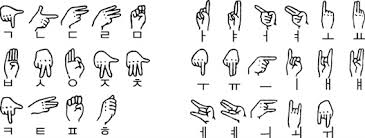
\includegraphics[scale=0.75]{images.jpg}
    \caption{자음 모음에 대응하는 지화}
  \end{figure}
 
\end{frame}

\begin{frame}{leap motion controller}
  
  \begin{itemize}
    \item leap motion회사에서 만든 두손과 손가락의 모든 움직임을 감지할 수 있는 USB 장치
  \end{itemize}
  \begin{figure}[h!]
    \centering
    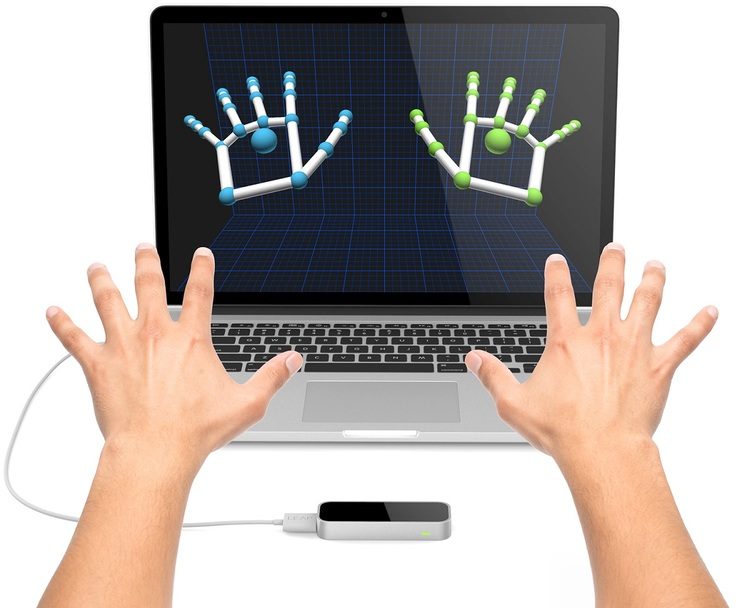
\includegraphics[scale=0.25]{2016120621586977.jpg}
    \caption{leap motion controller}
  \end{figure}

\end{frame}


\begin{frame}{}
  \begin{itemize}
    \item 주제 : 립모션 컨트롤러를 이용해 지화를 번역하는 어플리케이션 개발
    \item 번역 언어 : 한국어,영어
    \item 결과물 : 모바일 앱
    \item 사용언어 : java
    \item 사용기술 : 립모션 sdk
  \end{itemize}
\end{frame}

\begin{frame}{진행방식}
  \begin{enumerate}
    \item 립모션 컨트롤러 구입 및 sdk 세팅
    \item sdk 사용법 학습
    \item 일단 컴퓨터 프로그램상에서 돌아갈 수 있도록 프로그램 제작.
    \item 모바일 포팅
    \item 마무리
  \end{enumerate}
\end{frame}

\begin{frame}{예상되는 난관}
  \begin{enumerate}
    \item 립모션 컨트롤러 구입 및 sdk 세팅 : 컨트롤러 구입 갯수 및 절차, 기간
    \item sdk 사용법 학습 
    \begin{itemize}
      \item 만약 생각한 주제가 기술적으로 불가능한 경우
      \item 비대면에서의 테스트
    \end{itemize}
    \item 일단 컴퓨터 프로그램상에서 돌아갈 수 있도록 프로그램 제작.
    \item 모바일 포팅
    \item 마무리
  \end{enumerate}
\end{frame}


% 립모션이란
% 손가락 인식


% \begin{itemize}
%     \item 결과물 : 모바일 앱
%     \item 사용언어 : java
%     \item 사용기술(예상) : 립모션 sdk, openCV 
%     \item 한국어, 영어
% \end{itemize}

% 필요한 기술
% 간트차트

\end{document}